

Our pipeline comprises the following key components: dataset extraction, textual time series annotation, and comprehensive evaluation of the annotations (Figure \ref{fig:flowchart}).

\begin{figure}[!htbp] % 'r' for right, 'l' for left
    \centering
    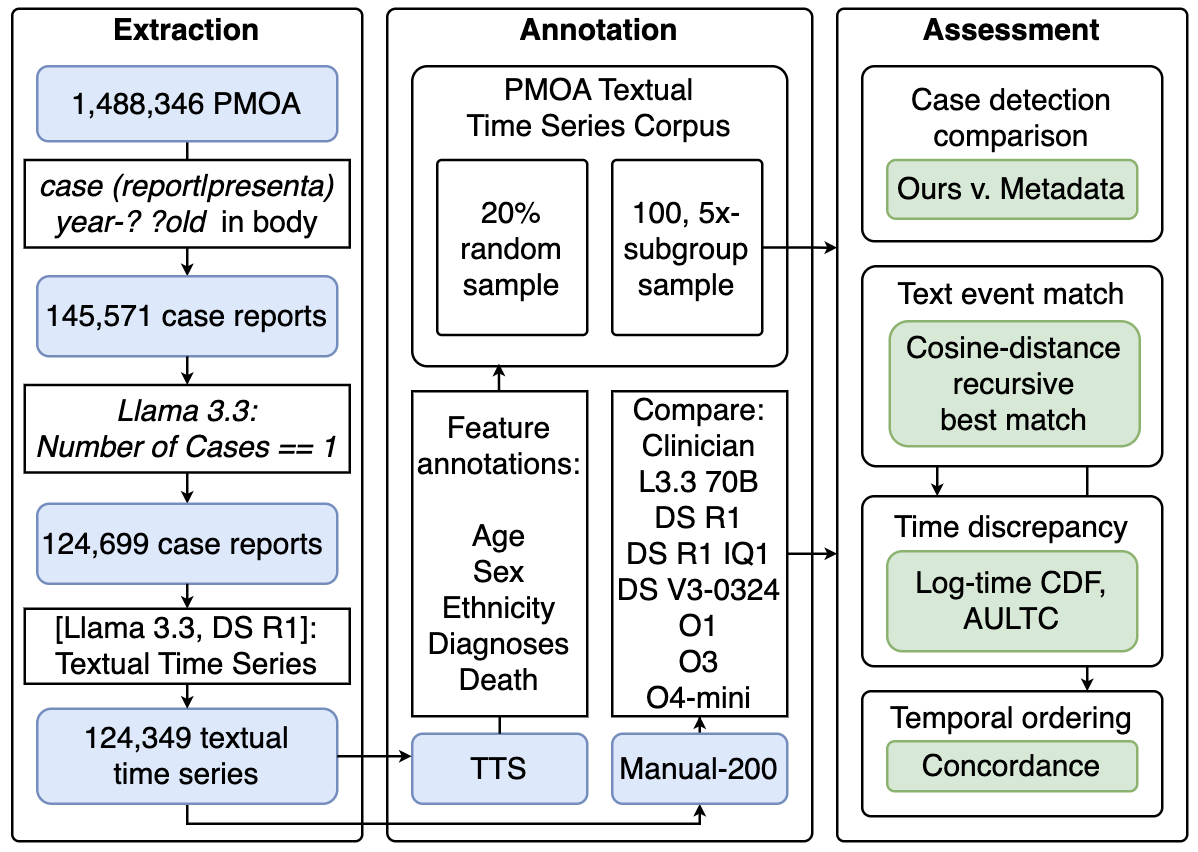
\includegraphics[width=0.75\linewidth]{Plots_tables/PMOATTS_flow5.png} % Adjust width
    \caption{Flowchart of the extraction and annotation pipeline. The left panel (Extraction) shows how we filtered the PMOA corpus to identify single-patient case reports. The middle panel (Annotation) depicts the generation of textual time series for each case via LLM prompting and the creation of evaluation subsets. The right panel (Assessment) summarizes the evaluation process, including metadata comparison, text event matching, time discrepancy analysis (log-time CDF, AULTC), and temporal order concordance. %\textbf{Right}: Age, sex, and ethnicity of the PMOA-TTS corpus. \textcolor{red}{Right figure missing? Remove/placeholder}
    }
    \label{fig:flowchart}
    \vspace{-2.5mm}
\end{figure}

\subsection{Case Report Identification Pipeline}

We use the PubMed Open Access (PMOA) repository data, which includes 1.4 million published manuscripts. Specifically, we utilize the plain text files from the December 17, 2024 release, located in the \texttt{oa\_noncomm} folder, which supports both noncommercial and commercial use. Following our previous work in \cite{wang2025large}, we identify candidate case reports by extracting content between the section markers ``\texttt{==== Body}'' and ``\texttt{==== Ref}'', which separate the main text and references in the PMOA format.

To ensure relevance, we first filter documents by matching the body text with the regular expressions ``\texttt{(case report|case presentation}'' and ``\texttt{year-? ?old}''. \textcolor{red}{George: In the regular expression "(case report|case presenta)" -- why "presenta"? If this is not a typo, it would be helpful to explain the reasoning here?}.
This filter yields 145,571 candidate documents likely to be case reports or case series. To narrow this set to single-patient case reports, we use a large language model (LLaMA 3.3 70B Instruct) to analyze each document's body text. The model is prompted with: ``\texttt{You are a physician. Determine the number of case reports in the following manuscript. Return 0 if it is not a case report. Reply only with the number and nothing else.}'', followed by the document body. We retain documents for which the model replies with \texttt{1} and discard others. This two-stage process results in a final dataset of 124,699 single-patient case reports (Figure~\ref{fig:flowchart}).

We compared our LLM-based case report identification method with PubMed's metadata-based labeling using a carefully designed benchmark. We created a dataset of 100 reports across five diagnoses—Diabetes, Sepsis, Hypertension, COVID-19, and Atrial Fibrillation—with 10 reports per diagnosis from each method. A clinician manually reviewed and labeled each report to verify whether it described exactly one case. 
%\textcolor{red}{Our LLM-pipeline significantly outperforms PubMed metadata filtering, particularly in terms of specificity and precision.}


%%%%%%%%%%%%%%%%%%%%%%%%%%%%
%%%%%%%%%%%%%%%%%%%%%%%%%%%%

\subsection{Timeline Annotation via LLM Prompting}

\subsubsection{Textual Time Series (TTS)}

We used LLMs (Llama 3.3, DeepSeek R1) to extract clinical textual time series from PMOA case reports. A textual time series is a chronologically ordered sequence of clinical findings, each associated with a timestamp and a specific patient. A clinical finding refers to a free-text description of a health-related condition affecting the patient. Our approach differs from conventional methods (e.g., \cite{sun2013evaluating, uzuner20112010}) by capturing longer, more context-rich text spans to accurately convey the meaning of clinical findings. Unlike the i2b2 guidelines, we do not limit findings to short prepositional phrases. For example, ``pain in chest that radiates substernally'' is kept intact to preserve its clinical nuance. Additionally, conjunctive findings are separated for clarity—e.g., ``metastases in the liver and pancreas'' is split into ``metastasis in the liver'' and ``metastasis in the pancreas.''

To construct clinical textual time series, we adopt the LLM extraction prompt from previous work \citep{wang2025large,noroozizadeh2025reconstructing}. This prompt instructs the LLM to extract clinical events with timestamps, setting the admission event at a reference time of 0, with other events expressed in relative hours (negative for pre-admission events, positive for post-admission). It also provides guidelines for handling conjunctions, event durations, and output formatting (full prompt shown below, \textbf{move to Appendix}).

\subsection{LLM Prompt to Generate Textual Time Series from PMOA Case Reports}
\label{apd:extraction-prompt}

% \begin{tcolorbox}[colback=gray!5, colframe=gray!100, title=LLM prompt to generate textual time series from PMOA case reports, boxrule=2pt]
\begin{tcolorbox}[
  colback=gray!5,
  colframe=gray!100,
  title=Prompt,
  boxrule=2pt,
  enhanced,
  breakable,                % <-- allows page breaks; starts here even if long
  before skip=8pt,          % spacing above (optional)
  after skip=8pt,           % spacing below (optional)
  pad at break*=2mm,        % padding at page break (optional)
  fontupper=\scriptsize,
  title after break={Prompt} % optional continuation note
]
You are a physician. Extract the clinical events and the related time stamp from the case report. The admission event has timestamp 0. If the event is not available, we treat the event, e.g. current main clinical diagnosis or treatment with timestamp 0. The events that happened before event with 0 timestamp have negative time, the ones after the event with 0 timestamp have positive time. The timestamp are in hours. The unit will be omitted when output the result. If there is no temporal information of the event, please use your knowledge and events with temporal expression before and after the events to provide an approximation. We want to predict the future events given the events happened in history. For example, here is the case report.\\

\textcolor{teal}{\texttt{An 18-year-old male was admitted to the hospital with a 3-day history of fever and rash. Four weeks ago, he was diagnosed with acne and received the treatment with minocycline, 100 mg daily, for 3 weeks. With increased WBC count, eosinophilia, and systemic involvement, this patient was diagnosed with DRESS syndrome. The fever and rash persisted through admission, and diffuse erythematous or maculopapular eruption with pruritus was present. One day later the patient was discharged.}}\\

Let's find the locations of events in the case report.
The phrase ‘a 3-day history of fever and rash’ directly places fever and rash 72 hours before admission, so both events receive timestamp \(-72\). The phrase ‘Four weeks ago’ directly places the acne diagnosis and initiation of minocycline treatment 672 hours before admission, so both events receive timestamp \(-672\). The diffuse erythematous or maculopapular eruption with pruritus is described in the admission context and is assigned timestamp 0. DRESS syndrome has no explicit timestamp, so clinical judgment is used to assign timestamp 0. The phrase ‘One day later’ places discharge 24 hours after admission.
% it shows that four weeks ago of fever and rash, four weeks ago, he was diagnosed with acne and receive treatment. So the event of fever and rash happened four weeks ago, 672 hours, it is before admitted to the hospital, so the time stamp is -672. diffuse erythematous or maculopapular eruption with pruritus was documented on the admission exam, so the timestamp is 0 hours, since it happens right at admission. DRESS syndrome has no specific time, but it should happen soon after admission to the hospital, so we use our clinical judgment to give the diagnosis of DRESS syndrome the timestamp 0. 
The output should look like:\\

%\vspace{2mm}
\texttt{18 years old | 0 \\
male | 0 \\
admitted to the hospital | 0 \\
fever | -72 \\
rash | -72 \\
acne | -672 \\
minocycline | -672 \\
increased WBC count | 0 \\
eosinophilia| 0 \\
systemic involvement| 0 \\
diffuse erythematous or maculopapular eruption| 0 \\
pruritis | 0 \\
DRESS syndrome | 0 \\
fever persisted | 0 \\
rash persisted | 0 \\
discharged | 24} \\

Separate conjunctive phrases into their component events and assign them the same timestamp (for example, separation of ‘fever and rash’ into 2 events: ‘fever’ and ‘rash’). If the event has duration, assign the event time as the start of the time interval. Attempt to use the text span without modifications except ‘history of’ where applicable. Include all patient events, even if they appear in the discussion; do not omit any events; include termination/discontinuation events; include the pertinent negative findings, like ‘no shortness of breath’ and ‘denies chest pain’. Show the events and timestamps in rows, each row has two columns: one column for the event, the other column for the timestamp. The time is a numeric value in hour unit. The two columns are separated by a pipe ‘|’ as a bar-separated file. Reply with the table only.
\end{tcolorbox}


For each report, the LLM generates a structured sequence of \mbox{(clinical event, time)} tuples. Events are retained in free-text form to preserve their clinical specificity, rather than being mapped to a fixed ontology. On average, each report contains 46 events, with significant variation depending on report length and complexity. The corpus as a whole includes over 5.6 million temporally anchored events, making it the largest public dataset of its kind in clinical NLP.

%%%%%%%%%%%%%%%%%%%%%%%%%%%%%%%%%%
\subsubsection{Sensitivity to Parts of the LLM Prompt Being Changed} \textcolor{red}{Move to Appendix?}

We slightly modified the prompt from the preceding section to check for sensitivity to specific parts of the LLM prompt being removed or modified.
% For sensitivity analyses with respect to the quality of different prompt strategies for extracting textual time series (\texttt{DeepSeek R1}) from PMOA case reports, we omitted selected sections of the LLM query prompt
% (see Appendix \ref{apd:extraction_prompt} for the full prompt).
This led to the following variants:
\begin{enumerate}
    \item \textbf{No changes}: Original LLM query prompt. % for \texttt{DeepSeek-R1}.
    
    \item \textbf{No role:} Remove the initial sentence \texttt{"You are a physician."}.
    
    \item \textbf{Zero-shot prompting:} Remove the example case report and textual time series from the prompt. \\
    %\item \textbf{No conjunction expansion:} 
    \textcolor{teal}{\texttt{An 18-year-old male was admitted to ..}}\\
    "Let's find the locations of event in the case report, it shows that ... then the output should look like:"\\
    \texttt{18 years old | 0 \\
    male | 0 \\
    ..}

    \item \textbf{No conjunction expansion:} Remove the following sentence from the prompt: \texttt{"Separate conjunctive phrases into its component events and assign them the same timestamp (for example, separation of ‘fever and rash’ into 2 events: ‘fever’ and ‘rash’)"}
    
    \item \textbf{Interval:} A query was added to the prompt for extracting the time interval (start and end time of clinical events). The original prompt’s instructions and few-shot examples were modified accordingly. 
    
    \item \textbf{Interval + Type:} A query was added to the prompt for extracting the time interval and i2b2
    event type (Interval+Type), where event type is one of: Factual, Possible, Hypothetical, Conditional, Negated, Historical, Uncertain. The original prompt’s instructions and few-shot examples were modified accordingly. 
\end{enumerate}


%%%%%%%%%%%%%%%%%%%%%%%%%%%
%%%%%%%%%%%%%%%%%%%%%%%%%%

\subsection{Manual Annotations}

We randomly sampled 180 case reports from PMOA--TTS and had them annotated by clinical experts. Combined with 20 manually annotated cases from our pilot study \citep{wang2025large}, the resulting set of 200 case reports serve as the gold standard for comparing LLM annotations against. 
The manual annotation process was conducted by expert physicians and followed the ISO-TimeML specification, which includes actions or states inferred to have occurred or held true. 
Annotators selected exact text spans representing events, with two exceptions to enhance usability: (i) conjunctive lists could be split into individual events, and (ii) the prefix ``history of'' could be added when contextually appropriate. \textcolor{red}{Jeremy: This was the request for the 20 annotations, but the request for the remaining 179 annotations was not this.  Sayantan has detailed annotation guidelines which can be used to rephrase this description} 
These adjustments preserved the original text alignment for downstream analysis. 
Each event was then assigned a time relative to the case reference point (e.g., admission or encounter date) \textcolor{red}{(George: is this case reference point not standardized? is there a way to have it be more standardized? I'd imagine if for some patients it's admission time whereas for others it is ``encounter date'', this would present challenges for downstream models used?)}, using the start time when an interval was described.
\textcolor{red}{George: Also state that (at least from my understanding) each case report is annotated by a single clinical expert? (If each case report was instead annotated by multiple experts, we should definitely indicate this to be the case.)}
We describe the evaluation metrics we use in the next section.
% This manually annotated subset of 200 cases serves as the gold standard for our evaluation metrics, described in the next section.

%%%%%%%%%%%%%%%%%%%%%%%%%%%
%%%%%%%%%%%%%%%%%%%%%%%%%%

\subsection{Evaluation Metrics} \textcolor{red}{Entire section move to Appendix?}

We assessed the textual time series extracted from PMOA case reports along three dimensions: (i) how well the extracted clinical events match up with manually annotated reference events (event match rate), (ii) how well the ordering of extracted clinical events matches that of the reference event ordering (temporal concordance), and (iii) how well extracted event times correspond to reference event times (time discrepancy). % using three key metrics: event match rate, temporal concordance (c-index), and log-time discrepancy.

\subsubsection{Event Match Rate}
%\textbf{Text Event Match.} 
To evaluate the alignment between predicted clinical events and reference annotations, we used a recursive best-match strategy adopted from our previous work \citep{wang2025large}. This method pairs events by minimizing string-based distances while avoiding many-to-one mappings. For each reference event, the closest predicted event is selected based on the minimal distance, with text order, \emph{i.e.}, the order of the events in the annotation files, to break distance ties. Once matched, both events are removed from further consideration, and the process continues recursively with the remaining pairs. \textcolor{red}{George: how does this greedy approach do compared to the classical 1955 Hungarian algorithm (we would use this to match predicted clinical events to reference ones, where if there is a mismatch in the numbers, e.g., more reference ones than predicted ones, you just introduce ``empty'' predicted ones that have 0 cost)? Also, is there some way to use an evaluation metric like optimal transport distance?}

We tested several distance metrics, including Levenshtein distance, cosine similarity of \texttt{BERT} (\texttt{bert-base-uncased}) embeddings, and cosine similarity based on sentence embeddings from \texttt{PubMedBERT} (\texttt{S-PubMedBert-MS-MARCO}). Previous validation showed that \texttt{PubMedBERT-based} cosine similarity with a threshold of 0.1 was the most reliable, and we used this metric for our evaluation. The detailed pseudo code of the recursive best match algorithm is provided in Algorithm~\ref{alg:recursive_match}. \textcolor{red}{George: Where does the threshold show up in Algorithm~1? How is the final event match rate defined (is it just the fraction of reference events that are matched, i.e., recall? precision? F1? something else?)?}
% We provide pseudocode for the best match procedure between two lists of strings (Algorithm \ref{alg:recursive_match}).  For each list, we use the text order, \emph{i.e.}, the order of the events in the annotation files, to break embedding distance ties.  We use the cosine similarity for the distance calculation using sentence transformer embeddings from \texttt{S-PubMedBert-MS-MARCO}.

\begin{algorithm}[ht]
\caption{Recursive Best Match}
\scriptsize
\label{alg:recursive_match}
\begin{algorithmic}[1]
\Require Two lists: \texttt{ref} (manually annotated reference events) and \texttt{pred} (predicted events)
\Ensure List of best-matching event pairs
\Function{MatchEvents}{\texttt{ref}, \texttt{pred}}
    \If{\texttt{ref} is empty \textbf{or} \texttt{pred} is empty}
        \State \Return \texttt{[]}
    \EndIf
    \State $\texttt{min\_distance} \gets \infty$
    \State $\texttt{best\_pair} \gets \texttt{None}$
    \ForAll{$r \in \texttt{ref}$}
        \ForAll{$p \in \texttt{pred}$}
            \State $d \gets \texttt{ComputeDistance}(r, p)$
            \If{$d < \texttt{min\_distance}$}
                \State $\texttt{min\_distance} \gets d$
                \State $\texttt{best\_pair} \gets (r, p)$
            \ElsIf{$d = \texttt{min\_distance}$}
                \State $(r^*, p^*) \gets \texttt{best\_pair}$
                \State Get indices (within the annotation files) of $r$, $p$, and also of $r^*, p^*$
                \If{index of $r <$ index of $r^*$}
                    \State $\texttt{best\_pair} \gets (r, p)$
                \ElsIf{index of $r = $ index of $r^*$ \textbf{and} index of $p <$ index of $p^*$}
                    \State $\texttt{best\_pair} \gets (r, p)$
                \EndIf
            \EndIf
        \EndFor
    \EndFor
    \State $(r^*,p^*) \gets \texttt{best\_pair}$
    \State Remove $r^*$ from \texttt{ref}
    \State Remove $p^*$ from \texttt{pred}
    \State $\texttt{result} \gets \texttt{[best\_pair]} + \texttt{MatchEvents}(\texttt{ref}, \texttt{pred})$
    \State \Return $\texttt{result}$
\EndFunction
\end{algorithmic}
\end{algorithm}

\subsubsection{Temporal Concordance}
%\textbf{Temporal Ordering.} 
To quantify the accuracy of temporal ordering, we used the concordance index (c-index), which measures the probability that a randomly selected pair of predicted events is correctly ordered in time (so c-index values range from 0 to 1). Higher c-index values indicate better alignment with the reference timeline. Formally, suppose that for a specific case report (corresponding to a single patient) that we have a manual annotation for, after doing the matching described in the previous section, we find that there are a total of $k$ events that matched. For event $i\in\{1,2,\dots,k\}$, we denote the (manually annotated) reference time for event $i$ as $t_i^{\text{ref}}$ and the LLM-extracted time as $t_p^{\text{pred}}$. Then the c-index is calculated as
\[
\text{c-index} = \frac{1}{N} \sum_{i,j\in\{1,2,\dots,k\}\text{ s.t.~}i<j} {\mathds{1}\{(t^{\text{ref}}_i - t^\text{ref}_j)(t^{\text{pred}}_i - t^{\text{pred}}_j) > 0\}},
\]
where $\mathds{1}\{\cdot\}$ is the indicator function, and $N$ is the number of ``comparable'' pairs (a pair of events $(i,j)$ with $i<j$ is comparable if $t^{\text{ref}}_i \neq t^{\text{ref}}_j$ and $t^{\text{pred}}_i \neq t^{\text{pred}}_j$).

% \vspace{-10pt}
% \begin{equation}
% \text{c-index} = \frac{1}{N} \sum_{i<j} \mathbf{1}[(t^r_i - t^r_j)(t^p_i - t^p_j) > 0]
% \end{equation}
% \vspace{-10pt}

\subsubsection{Time Discrepancy}
%\textbf{Time Discrepancy Analysis.} 
We evaluated temporal prediction accuracy by measuring the discrepancies between predicted and reference times. Continuing to use notation from the previous section, note that for a specific matched event, the absolute difference in predicted and reference times is $|t_i^{\text{pred}} - t_i^{\text{ref}}|$. If we denote any such absolute time difference as $\Delta t$ (in hours), then we specifically measure the \emph{log-time discrepancy} defined as $\log(1 + \Delta t)$. To summarize these discrepancies, we introduce the Area Under the Log-Time Cumulative Distribution Function (AULTC), which quantifies how quickly the cumulative distribution of log-time discrepancy values rises---higher AULTC values indicate better temporal alignment. The full definition of AULTC is in Appendix \ref{apd:ltcdf}. We also stratified the analysis by different time granularities (hour, day, week, year) to examine how prediction accuracy varies with time from case presentation. \textcolor{red}{George: In constructing the empirical distribution function, do you use log-time discrepancy values across the entire ``gold set''?}

%%%%%%%%%%%%%%%%%%%%%%%%%%%
%%%%%%%%%%%%%%%%%%%%%%%%%%

\subsection{Computational Resources for Reproducibility}
We designed the PMOA–TTS pipeline to ensure reproducibility and transparency across all stages of extraction, annotation, and evaluation. All experiments and annotations involving large language models (LLMs) were executed using commercially available APIs (OpenAI) or open-source models run on GPU-accelerated infrastructure (HuggingFace).

\texttt{DeepSeek-R1} was run on an 6$\times$NVIDIA H200 GPUs. Inference for \texttt{DeepSeek-R1-IQ1} and \texttt{LLaMA 3.3–70B} were performed using Hugging Face’s transformers library on a 2$\times$A100 GPU setup. Each inference pass over a full case report required between 10 to 120 seconds per document depending on model size, context length, and prompt complexity. Total timeline extraction across 124,699 reports took approximately 8400 GPU-hours on \texttt{DeepSeek-R1} and 2000 GPU-hours for \texttt{LLaMA 3.3–70B}.  Temperature was set to recommended levels of 0.6 for \texttt{DeepSeek} models, and 0.7 for \texttt{Llama 3.3-70B}.
Experiments using OpenAI  models were conducted via the Azure OpenAI API.
% , and we used temperature=0 settings for deterministic behavior \textcolor{red}{Do we say anything about the random seeds?}. \jeremy{we don't have access to a temperature setting for OpenAI.}
